


\documentclass[conference]{IEEEtran}
\IEEEoverridecommandlockouts
% The preceding line is only needed to identify funding in the first footnote. If that is unneeded, please comment it out.
\usepackage{cite}
\usepackage{amsmath,amssymb,amsfonts}
\usepackage{algorithmic}
\usepackage{graphicx}
\usepackage{stfloats}
\usepackage{textcomp}
\usepackage{xcolor}
\usepackage{multirow}
\def\BibTeX{{\rm B\kern-.05em{\sc i\kern-.025em b}\kern-.08em
    T\kern-.1667em\lower.7ex\hbox{E}\kern-.125emX}}
\begin{document}

% MDP 、MCRA添加参考文献
%index 部分结尾处要不要添加 。
%figure reports -> shows
% future work 改被动式
% 主动换被动
% 避免中式英语-结论部分

\title{HD-MCRA: Hierarchical Reach-Avoid Navigation for Quadruped Robots}

\author{\IEEEauthorblockN{1\textsuperscript{st} Given Name Surname}
\IEEEauthorblockA{\textit{dept. name of organization (of Aff.)} \\
\textit{name of organization (of Aff.)}\\
City, Country \\
email address or ORCID}
\and
\IEEEauthorblockN{2\textsuperscript{nd} Given Name Surname}
\IEEEauthorblockA{\textit{dept. name of organization (of Aff.)} \\
\textit{name of organization (of Aff.)}\\
City, Country \\
email address or ORCID}
\and
\IEEEauthorblockN{3\textsuperscript{rd} Given Name Surname}
\IEEEauthorblockA{\textit{dept. name of organization (of Aff.)} \\
\textit{name of organization (of Aff.)}\\
City, Country \\
email address or ORCID}
}

\maketitle

\begin{abstract}
This paper addresses quadruped robot navigation subject to safety and efficiency requirements. We formulate the task as a minimum-cost reach-avoid problem, where the robot must reach the goal without entering unsafe sets while minimizing cumulative execution cost. To address this challenge, we propose HD-MCRA, which combines a frozen robust low-level velocity tracker that induces a stable high-level abstraction with data-driven conservative margins that compensate for residual execution mismatch, thereby enabling effective budget-conditioned reach-avoid learning. Simulation results show that HD-MCRA consistently provides a more favorable trade-off among task success, safety, budget feasibility, clearance, and navigation cost than existing baselines.
\end{abstract}

\begin{IEEEkeywords}
quadruped robot, navigation, reach-avoid, hierarchical reinforcement learning, safe reinforcement learning
\end{IEEEkeywords}

\section{Introduction}
Recent advances in learning-based quadruped locomotion have substantially improved agile motion and terrain adaptation on physical robots \cite{DBLP:journals/scirobotics/HwangboWK020,DBLP:conf/rss/KumarFPM21,DBLP:journals/scirobotics/MikiLHWKH22}. As a result, the primary deployment bottleneck has shifted from low-level locomotion capability to high-level autonomous navigation in cluttered environments. In practical missions such as inspection, search and rescue, and security patrol, quadruped navigation must satisfy two hard requirements simultaneously: collision-free goal reaching and low execution cost under contact-rich execution and perception uncertainty.

Existing methods do not fully address this combined objective. Classical planners such as DWA and D* Lite \cite{DBLP:journals/ram/FoxBT97,DBLP:conf/aaai/KoenigL02} rely on modeling and execution assumptions that are difficult to maintain on quadruped platforms. In contrast, many reinforcement learning approaches optimize weighted rewards or constrained objectives \cite{DBLP:conf/icml/AchiamHTA17,DBLP:conf/iclr/TesslerMM19,DBLP:journals/ral/YuanHZBGPS22}, which either relax safe goal-reaching into a tunable preference or introduce sensitivity to constraint-threshold selection. A more suitable formulation is the \emph{minimum-cost reach-avoid} (MCRA) problem, where safe goal-reaching is enforced as a trajectory-level constraint while execution cost is minimized. Recent reach-avoid methods and the budget-conditioned RC-PPO framework \cite{DBLP:conf/rss/HsuRTF21,DBLP:conf/nips/SoGF24} provide a principled approach to cost-aware policy learning. However, RC-PPO assumes deterministic dynamics, which precludes commonly used deployment-oriented techniques such as domain randomization and limits its direct applicability to quadruped navigation.

To address these issues, we propose \emph{HD-MCRA} (\emph{Hierarchical Data-driven Minimum-Cost Reach-Avoid}), a hierarchical minimum-cost reach-avoid framework with data-driven conservative margins for quadruped navigation. We first train a robust low-level velocity tracker with PPO under domain randomization and then freeze it to induce an approximately deterministic interface for high-level learning. On top of this interface, we learn a high-level budget-conditioned reach-avoid policy over low-dimensional velocity commands and introduce two data-driven conservative margins, $\alpha$ and $\delta$, to compensate for budget overrun and trajectory deviation. 

The main contributions are twofold: 1) we formulate quadruped navigation as an MCRA problem to explicitly encode both safe goal-reaching and cost minimization; and 2) we develop a hierarchical MCRA framework with data-driven conservative margins, making budget-conditioned minimum-cost reach-avoid learning practical for quadruped robots.





















\section{Problem Formulation}
To formalize quadruped navigation in cluttered environments, we model the high-level decision-making process as a Markov decision process (MDP)
\begin{equation}
\mathcal{M}=\langle \mathcal{X}, \mathcal{U}^{\mathrm{high}}, P, c, \rho_0 \rangle
\end{equation}
where $\mathcal{X}$ denotes the high-level state space, $\mathcal{U}^{\mathrm{high}}$ denotes the action space of commanded base velocities, $P(\cdot|x_t,u_t)$ denotes the transition kernel, $c(x_t,u_t)$ denotes the instantaneous execution cost, and $\rho_0$ denotes the initial-state distribution. At the navigation level, the state $x_t$ contains the information required for safe decision making, including local environmental observations and the robot's navigation state, while the high-level action $u_t \in \mathcal{U}^{\mathrm{high}}$ is a low-dimensional velocity command.

Let $\mathcal{G}\subseteq\mathcal{X}$ be the goal set and $\mathcal{F}\subseteq\mathcal{X}$ be the unsafe set induced by collision or safety violation. Starting from an initial state $x_0$, the task is to find a policy $\pi$ and a free terminal time $T$ such that the robot reaches $\mathcal{G}$, avoids $\mathcal{F}$ throughout the trajectory, and minimizes the cumulative cost. Accordingly, the quadruped navigation task is formulated as a minimum-cost reach-avoid (MCRA) problem:
\begin{align}
\min_{\pi,T}\quad & \sum_{t=0}^{T-1} c\!\left(x_t,\pi(x_t)\right) \label{eq:mcra_obj}\\
\mathrm{s.t.}\quad & x_T \in \mathcal{G}, \label{eq:mcra_goal}\\
& x_t \notin \mathcal{F},\quad \forall t\in\{0,\dots,T\}, \label{eq:mcra_safe}\\
& x_{t+1}\sim P\!\left(\cdot\mid x_t,\pi(x_t)\right). \label{eq:mcra_dyn}
\end{align}
The goal and unsafe sets are represented by two signed functions
$g:\mathcal{X}\rightarrow\mathbb{R}$ and $h:\mathcal{X}\rightarrow\mathbb{R}$ as
\begin{equation}
\mathcal{G} := \{x\in\mathcal{X}\mid g(x)\le 0\}
\end{equation}
\begin{equation}
\mathcal{F} := \{x\in\mathcal{X}\mid h(x)>0\}
\end{equation}
This formulation differs fundamentally from reward shaping: goal-reaching and safety are treated as trajectory-level constraints rather than encoded as soft preferences through weighted rewards. For quadruped navigation, this distinction is important because surrogate reward or CMDP objectives may not align with the true requirement of safe arrival with minimum cumulative cost \cite{DBLP:conf/nips/SoGF24}.

RC-PPO addresses the minimum-cost reach-avoid problem by augmenting the system state with variables that encode the safety status and remaining budget, thereby recasting the original problem as a reachability problem on an augmented state space \cite{DBLP:conf/nips/SoGF24}. This augmented-state construction was developed for deterministic discrete-time dynamics of the form $x_{t+1}=f(x_t,u_t)$, rather than for the stochastic dynamics in \eqref{eq:mcra_dyn}. We therefore first recall the augmented-state representation used in that deterministic setting. 

Define the augmented state as
\begin{equation}
\hat{x}_t=(x_t,y_t,z_t)\in \hat{\mathcal{X}}:=\mathcal{X}\times\{-1,1\}\times\mathbb{R}
\end{equation}
where $y_t$ is a binary safety indicator and $z_t$ is a remaining cost budget. The corresponding augmented dynamics are
\begin{equation}
\begin{aligned}
\hat{f}(x_t,y_t,z_t,u_t)
= \big(&f(x_t,u_t), \\
&\max\{I_{f(x_t,u_t)\in\mathcal{F}},y_t\}, \\
&z_t-c(x_t,u_t)\big)
\end{aligned}
\end{equation}
where $I_{b\in\mathcal{B}}$ is the shifted indicator. By construction, $z_t$ evolves as
\begin{equation}
z_{t+1}=z_0-\sum_{k=0}^{t} c(x_k,u_k)
\end{equation}
which means that $z_0$ serves as an upper bound on the cumulative cost incurred along the trajectory. Then the augmented goal function can be defined as
\begin{equation}
\hat{g}(x,y,z)=\max\{g(x),Cy,-z\}
\end{equation}
with augmented goal set
\begin{equation}
\begin{aligned}
\hat{\mathcal{G}}
&=\{\hat{x}\mid \hat{g}(\hat{x})\le 0\} \\
&=\{(x,y,z)\mid x\in\mathcal{G},\, y=-1,\, z\ge 0\}
\end{aligned}
\end{equation}
Under this construction, reaching $\hat{\mathcal{G}}$ implies that the original system reaches the goal, remains safe along the whole trajectory, and does not exceed the prescribed budget, which is the key theoretical bridge from reach-avoid constraints to cost-aware reachability \cite{DBLP:conf/nips/SoGF24}.

Therefore, the corresponding MCRA problem in the deterministic setting can be equivalently interpreted as searching for the least feasible initial budget
\begin{align}
\min_{\pi,z_0}\quad & z_0 \\
\mathrm{s.t.}\quad & \tilde{V}^{\pi}_{\hat{g}}(x_0,I_{x_0\in\mathcal{F}},z_0)\le 0,
\end{align}
where $\tilde{V}^{\pi}_{\hat{g}}$ is the reach value function on the augmented system. However, this deterministic reformulation is not yet sufficient for quadruped navigation: the real closed-loop system remains stochastic, contact-rich, and subject to execution variability, and robustness tools such as domain randomization do not fit directly into the deterministic assumptions behind RC-PPO. Bridging this gap requires a quadruped-specific nominal closed-loop abstraction together with conservative corrections to account for residual mismatch, which motivates the HD-MCRA framework introduced next.







\section{HD-MCRA}
\subsection{Framework Overview}
HD-MCRA makes minimum-cost reach-avoid learning practical for quadruped robots by separating navigation-level decision making from locomotion execution. We first train a low-level policy under domain randomization to robustly track commanded base velocities and then freeze it as a motion interface. Given this fixed interface, a high-level policy receives local perception, task observations, and the remaining budget, and outputs low-dimensional velocity commands. This hierarchy avoids end-to-end joint-space learning, preserves locomotion feasibility, and provides the high-level policy with a more stationary closed-loop system for budget-conditioned MCRA learning; residual mismatch in this nominal interface is addressed by the conservative margins $\alpha$ and $\delta$.

Formally, let the overall policy be written as
\begin{equation}
u_t^{\mathrm{joint}}
=\pi^{\mathrm{low}}\big(s_t^{\mathrm{low}},u_t^{\mathrm{high}}\big)
\end{equation}
\begin{equation}
u_t^{\mathrm{high}}
=\pi^{\mathrm{high}}(o_t,z_t)
\end{equation}
where $o_t$ denotes the high-level observation, $u_t^{\mathrm{high}}$ denotes the commanded base velocity, $s_t^{\mathrm{low}}$ denotes the low-level locomotion state, and $u_t^{\mathrm{joint}}$ denotes the final joint-level control action. This factorization allows the navigation problem to be solved in a lower-dimensional action space while preserving the physical feasibility of locomotion execution.

\subsection{Hierarchical Budgeted Policy Learning}

The low-level controller maps proprioceptive observations to actuator commands to track high-level velocity commands while preserving locomotion stability. Its state is $s_t^{\mathrm{low}} \in \mathcal{S}^{\mathrm{low}}$, which includes joint positions, joint velocities, body orientation, angular velocity, and recent tracking information, and its action is the joint-level command $u_t^{\mathrm{joint}} \in \mathcal{U}^{\mathrm{joint}}$. Given a commanded base velocity
\begin{equation}
u_t^{\mathrm{high}} = \big[v_{x,t}^{\ast}, v_{y,t}^{\ast}, \omega_{z,t}^{\ast}\big]^{\top}
\end{equation}
the controller aims to minimize tracking error while maintaining stable motion.

We train this controller with PPO under domain randomization \cite{DBLP:journals/corr/SchulmanWDRK17,DBLP:conf/iros/TobinFRSZA17}. Let $\bar{u}_t^{\mathrm{body}}=[v_{x,t},v_{y,t},\omega_{z,t}]^{\top}$ denote the realized body velocity. The reward combines velocity-tracking, control-smoothness, and posture-stability terms:
\begin{equation}
\begin{aligned}
r_t^{\mathrm{low}}
=\,&-\lambda_v \left\| \bar{u}_t^{\mathrm{body}}-u_t^{\mathrm{high}} \right\|_2^2 \\
&-\lambda_u \left\| u_t^{\mathrm{joint}} \right\|_2^2 -\lambda_p \phi_t^{\mathrm{stab}}
\end{aligned}
\end{equation}
where $\phi_t^{\mathrm{stab}}$ penalizes unstable motions such as excessive roll, pitch, or slippage. Randomizing dynamics and terrain parameters improves robustness, and the trained $\pi^{\mathrm{low}}$ is frozen before high-level learning.

With this motion interface fixed, the high-level policy solves the navigation problem using the minimum-cost reach-avoid formulation introduced in Section II. Let the high-level observation be $o_t \in \mathcal{O}$, which contains local LiDAR-based obstacle information, relative goal information, and robot navigation state. The high-level action is the commanded base velocity
\begin{equation}
u_t^{\mathrm{high}}=\pi^{\mathrm{high}}(o_t,z_t)
\end{equation}
where $z_t$ is the remaining budget variable. With the low-level controller frozen, the high-level process induces a reduced closed-loop transition kernel $P_{\mathrm{cl}}(\cdot\mid x_t,u_t^{\mathrm{high}})$. We approximate this kernel with a nominal closed-loop map and write
\begin{equation}
x_{t+1}=\bar{f}_{\mathrm{cl}}\!\left(x_t,\pi^{\mathrm{high}}(o_t,z_t)\right)
\end{equation}
for high-level training, where $\bar{f}_{\mathrm{cl}}$ denotes the nominal closed-loop abstraction obtained by composing the robot dynamics with the frozen low-level tracker. Domain-randomized rollouts indicate that this closed-loop kernel is substantially more concentrated than the transition distribution induced by end-to-end joint-space control, making the nominal abstraction useful at the navigation level.

The high-level policy is conditioned on the remaining budget $z_t$, so that one policy can adapt to different cost-feasibility levels. Intuitively, larger budgets permit more conservative maneuvers, whereas tighter budgets encourage shorter and more efficient motion, provided that safety is preserved.

The high-level objective is to learn a policy that safely reaches the goal within feasible cost budgets while enabling the search for the minimum feasible initial budget:
\begin{align}
\min_{\pi^{\mathrm{high}}, z_0}\quad & z_0 \\
\mathrm{s.t.}\quad &
x_T \in \mathcal{G}, \;
x_t \notin \mathcal{F}, \ \forall t\le T .
\end{align}

\noindent\textbf{Assumption 1 (Concentrated closed-loop abstraction).}
With the low-level tracker frozen, the induced high-level closed-loop transition kernel is concentrated around $\bar{f}_{\mathrm{cl}}$. In particular, the one-step deviation
\(
e_t:=x_{t+1}-\bar{f}_{\mathrm{cl}}(x_t,u_t^{\mathrm{high}})
\)
and the relative cost overrun ratio admit bounded upper quantiles under domain-randomized rollouts.

\subsection{Data-driven Robustness Margins}

Although the frozen low-level controller provides a more stable interface, real-world quadruped deployment still exhibits residual mismatch between simulated and realized trajectories. Two typical failure modes are especially important. First, due to tracking delays or locomotion disturbances, the realized execution cost may exceed the planned budget, causing a nominally feasible trajectory to violate the cost constraint. Second, due to body oscillation or lateral deviation, the realized robot trajectory may pass closer to obstacles than expected, resulting in a collision even when the nominal high-level plan is safe.

To address these issues, we introduce two conservative margins: a \emph{cost margin} $\alpha$ and a \emph{safety margin} $\delta$. These margins account for stochastic execution mismatch by yielding a robustified nominal MCRA problem. The cost margin is used to inflate the effective running cost:
\begin{equation}
\tilde{c}^{\mathrm{high}}(x_t,u_t^{\mathrm{high}})
=(1+\alpha)\, c^{\mathrm{high}}(x_t,u_t^{\mathrm{high}})
\end{equation}
so that the high-level budget update becomes
\begin{equation}
z_{t+1}=z_t-\tilde{c}^{\mathrm{high}}(x_t,u_t^{\mathrm{high}})
\end{equation}
This design reserves additional budget to account for cost overruns caused by execution mismatch. The safety margin is used to shrink the feasible free space or, equivalently, enlarge the unsafe set:
\begin{equation}
\mathcal{F}_{\delta}=\{x\in\mathcal{X}\mid d(x,\mathcal{F})\le \delta\}
\end{equation}
where $d(x,\mathcal{F})$ denotes the distance from the state to the unsafe set. By replacing $\mathcal{F}$ with $\mathcal{F}_{\delta}$ during training and deployment, the policy is encouraged to maintain greater clearance from obstacles and becomes more robust to lateral tracking deviations.

Importantly, $\alpha$ and $\delta$ are not manually selected as heuristic constants. Instead, they are estimated from domain-randomized rollout statistics obtained with the frozen low-level controller. Let $\varepsilon_c$ denote the relative cost overrun ratio between actual and nominal execution, and let $\varepsilon_d$ denote the trajectory deviation with respect to the nominal body path. We select $\alpha$ and $\delta$ from suitable upper quantiles of their empirical distributions:
\begin{equation}
\alpha = Q_{p_c}(\varepsilon_c)
\end{equation}
\begin{equation}
\delta = Q_{p_d}(\varepsilon_d)
\end{equation}
where $Q_{p}(\cdot)$ denotes the empirical $p$-quantile. The nominal MCRA problem is therefore solved on an uncertainty-aware surrogate model: the transition is represented by $\bar{f}_{\mathrm{cl}}$, the unsafe set is enlarged by $\delta$, and the running cost is inflated by $\alpha$. In this way, both margins are data-driven and directly derived from the residual stochasticity observed under randomized conditions.

\noindent\textbf{Proposition 1 (Quantile-based robustness).}
If a nominal trajectory generated by $\bar{f}_{\mathrm{cl}}$ reaches $\mathcal{G}$ while remaining outside $\mathcal{F}_{\delta}$ and satisfying the inflated budget update with $\tilde{c}^{\mathrm{high}}$, then the realized trajectory is safe and budget-feasible whenever the tracking deviation and cost overrun stay within the empirical quantiles used to define $\delta$ and $\alpha$. 

\subsection{Two-phase Solver}

Under this robustified formulation, the high-level policy is trained using a two-phase RL procedure. In \emph{Phase I}, we train a stochastic policy $\pi_\theta^{\mathrm{high}}(u\mid o,z)$ together with a reachability critic on the augmented state $\hat{x}_t=(x_t,y_t,z_t)$. On the closed-loop abstraction, the critic is trained with the discounted reachability target
\begin{equation}
\begin{aligned}
\tilde{V}_{\psi}(\hat{x}_t)
=\,&(1-\gamma)\hat{g}(\hat{x}_t) \\
&+\,\gamma\, \mathbb{E}\!\left[
\min\!\left\{\hat{g}(\hat{x}_t),\tilde{V}_{\psi}(\hat{x}_{t+1})\right\}
\right]
\end{aligned}
\end{equation}
where $\hat{g}(x,y,z)=\max\{g(x),Cy,-z\}$ and $\hat{x}_{t+1}$ is generated by $\bar{f}_{\mathrm{cl}}$. During training, the initial budget $z_0$ is sampled from a prescribed interval $[z_{\min},z_{\max}]$, and the actor is updated with PPO using the resulting advantage estimates.

In \emph{Phase II}, the stochastic actor is converted into a deterministic deployment policy using its mean action, and the value function is re-evaluated under the uncertainty-aware model defined by $\tilde{c}^{\mathrm{high}}$ and $\mathcal{F}_{\delta}$. The minimum feasible initial budget is then obtained by a one-dimensional search over $z_0$ for the start state or start-state distribution. In this way, the two-phase solver extends budget-conditioned reach-avoid learning to quadruped navigation by leveraging the frozen low-level interface and data-driven robustness margins.




























\section{Experiments and Results}

\subsection{Experimental Setup}

We evaluate \emph{HD-MCRA} on quadruped navigation in cluttered environments, where the robot uses local obstacle observations and goal-relative information to generate commanded body velocities for safely reaching the target while minimizing cumulative cost. The test suite covers three difficulty levels: moderately cluttered scenes, narrow passages, and densely obstructed scenes.

We compare HD-MCRA with four families of baselines: a \emph{reach-avoid baseline} (RA) \cite{DBLP:conf/rss/HsuRTF21}, a \emph{minimum-cost reach-avoid baseline} (RC-PPO) \cite{DBLP:conf/nips/SoGF24}, reward-shaped PPO, and CPPO with two safety weights ($\beta_L,\beta_H$). To ensure a fair comparison, all methods use the same high-level observations, commanded-velocity action interface, frozen low-level tracker, and training/evaluation maps \cite{DBLP:conf/icml/AchiamHTA17,DBLP:conf/iclr/TesslerMM19,DBLP:journals/ral/YuanHZBGPS22,DBLP:journals/ral/HuZTRAN21,DBLP:conf/icra/WeerakoonSEM24}. We report Success Rate (SR), Collision Rate (CR), Average Cost, Budget Violation Rate (BVR), and Minimum Clearance (MC).

\subsection{Baseline Comparison}

Figure~\ref{fig:metrics_grid_single_column} shows the scenario-wise comparison in terms of SR, CR, Average Cost, and MC. Table~\ref{tab:main_result} summarizes the average performance over the three scenarios and also reports BVR.

\begin{figure}[t]
\centering
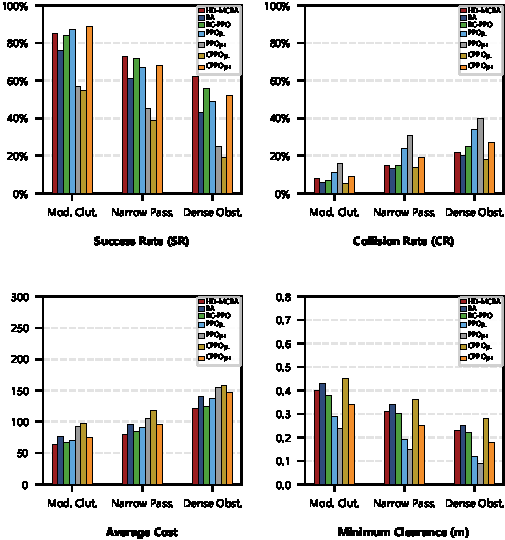
\includegraphics[width=\columnwidth]{figures_v3/figure_metrics_grid_single_column_v3}
\caption{Performance comparison across three navigation scenarios. From top-left to bottom-right: success rate, collision rate, average cost, and minimum clearance.}
\label{fig:metrics_grid_single_column}
\end{figure}


\begin{table}[t]
\caption{Average performance over the three scenarios.}
\label{tab:main_result}
\centering
\resizebox{\columnwidth}{!}{%
\begin{tabular}{lccccc}
\hline
Method & SR (\%) $\uparrow$ & CR (\%) $\downarrow$ & Cost $\downarrow$ & BVR (\%) $\downarrow$ & MC (m) $\uparrow$ \\
\hline
HD-MCRA & 73.3 & 15.0 & 88.3 & 9.0 & 0.31 \\
RA & 60.0 & 13.0 & 104.0 & 20.0 & 0.34 \\
RC-PPO & 70.7 & 15.7 & 91.7 & 14.0 & 0.30 \\
PPO$_{\beta L}$ & 67.7 & 23.0 & 99.7 & 20.7 & 0.20 \\
PPO$_{\beta H}$ & 42.3 & 29.0 & 117.0 & 27.0 & 0.16 \\
CPPO$_{\beta L}$ & 37.7 & 12.3 & 124.7 & 22.3 & 0.36 \\
CPPO$_{\beta H}$ & 69.7 & 18.3 & 105.7 & 17.0 & 0.26 \\
\hline
\end{tabular}}
\end{table}

Figure~\ref{fig:metrics_grid_single_column} and Table~\ref{tab:main_result} indicate that HD-MCRA achieves the most balanced overall performance across task completion, safety, budget feasibility, and efficiency in the three scenarios. Relative to RA, HD-MCRA achieves a higher success rate and lower cost while maintaining comparable safety. Compared with RC-PPO, HD-MCRA further improves budget feasibility and slightly increases minimum clearance, while also attaining the best average success rate. The PPO/CPPO baselines exhibit the usual trade-off: some settings remain competitive in easier scenes or improve clearance, but none matches HD-MCRA in terms of success, budget feasibility, and efficiency simultaneously.

\subsection{Budget Feasibility Analysis}

To directly evaluate budget sensitivity, we sweep the normalized initial budget $z_0/z_{\mathrm{ref}}$ over $\{0.80,0.85,0.90,0.96,1.00,1.05,1.12,1.20\}$, where $z_{\mathrm{ref}}$ denotes a scenario-dependent reference feasible budget. Figure~\ref{fig:budget_sweep} reports the resulting SR, CR, BVR, and navigation cost curves for RA, RC-PPO, and HD-MCRA.

\begin{figure}[t]
\centering
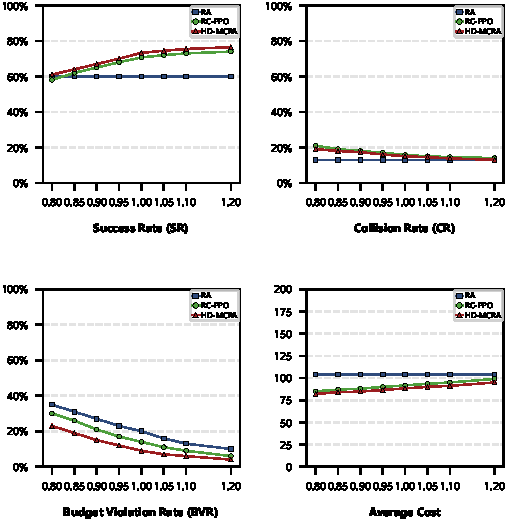
\includegraphics[width=\columnwidth]{figures_v3/figure_budget_sweep_v3}
\caption{Budget-response curves under normalized initial budgets.}
\label{fig:budget_sweep}
\end{figure}


RA is largely budget-agnostic: its SR, CR, and Average Cost remain almost unchanged across the sweep, and only BVR decreases as the budget is relaxed. In contrast, RC-PPO and HD-MCRA exhibit clear budget-response behavior, achieving higher SR and lower CR and BVR as the budget increases. HD-MCRA remains more reliable than RC-PPO even under tight budgets: at $z_0/z_{\mathrm{ref}}=0.90$, it achieves $66.8\%$ SR with $14.7\%$ BVR, whereas RC-PPO requires a larger budget to achieve comparable feasibility.

To formalize the search for the least feasible initial budget, we define
\begin{equation}
\begin{aligned}
z_0^\star
= \min \Big\{ z_0 \;\Big|\; &\mathrm{SR}\ge 60\%,\; \mathrm{CR}\le 20\%, \\
&\mathrm{BVR}\le 15\% \Big\}
\end{aligned}
\end{equation}
where the criteria are evaluated on the complete test set. Table~\ref{tab:min_budget} shows that HD-MCRA achieves the smallest feasible budget, $z_0^\star/z_{\mathrm{ref}}=0.90$, compared with $0.96$ for RC-PPO and $1.12$ for RA. This is the clearest evidence that budget conditioning is necessary for cost-feasible navigation and that the conservative margins improve robustness under execution uncertainty.

\begin{table}[t]
\caption{Search result for the minimum feasible normalized initial budget.}
\label{tab:min_budget}
\centering
\resizebox{\columnwidth}{!}{%
\begin{tabular}{lcccc}
\hline
Method & $z_0^\star / z_{\mathrm{ref}}$ $\downarrow$ & SR@${z_0^\star}$ (\%) $\uparrow$ & CR@${z_0^\star}$ (\%) $\downarrow$ & BVR@${z_0^\star}$ (\%) $\downarrow$ \\
\hline
HD-MCRA & 0.90 & 66.8 & 17.6 & 14.7 \\
RC-PPO & 0.96 & 62.9 & 18.8 & 14.9 \\
RA & 1.12 & 60.5 & 13.7 & 14.4 \\
\hline
\end{tabular}}
\end{table}

Taken together, Figure~\ref{fig:budget_sweep} and Table~\ref{tab:min_budget} show that RA does not adapt to budget, RC-PPO captures the benefit of budget conditioning, and HD-MCRA reaches feasibility at the smallest budget.

\subsection{Ablation Study}

To further understand the role of each design component, we conduct ablation studies on the hierarchical structure and the two conservative margins. The variants compared are: 1) the full HD-MCRA framework, 2) a version without hierarchical decomposition (\emph{w/o Hierarchy}), 3) a version without the cost margin $\alpha$, 4) a version without the safety margin $\delta$, and 5) a version without both margins (\emph{w/o $\alpha,\delta$}), while retaining the hierarchical budget-conditioned policy. The ablation study is conducted on a separate controlled evaluation batch dedicated to component analysis; therefore, the absolute values in Table~\ref{tab:ablation} are intended for within-table comparison and should not be directly compared with those in Table~\ref{tab:main_result}.

\begin{table}[t]
\caption{Ablation study on hierarchy and conservative margins.}
\label{tab:ablation}
\centering
\resizebox{\columnwidth}{!}{%
\begin{tabular}{lccccc}
\hline
Variant & SR (\%) $\uparrow$ & CR (\%) $\downarrow$ & Cost $\downarrow$ & BVR (\%) $\downarrow$ & MC (m) $\uparrow$ \\
\hline
w/o Hierarchy & 47.9 & 38.8 & 116.7 & 31.5 & 0.11 \\
w/o $\alpha$ & 67.2 & 19.8 & 80.6 & 22.4 & 0.29 \\
w/o $\delta$ & 64.8 & 26.3 & 77.2 & 13.8 & 0.19 \\
w/o $\alpha,\delta$ & 62.9 & 29.4 & 87.6 & 25.8 & 0.16 \\
HD-MCRA (full) & 70.8 & 18.6 & 71.3 & 11.2 & 0.32 \\
\hline
\end{tabular}}
\end{table}

\begin{figure*}[!t]
\centering
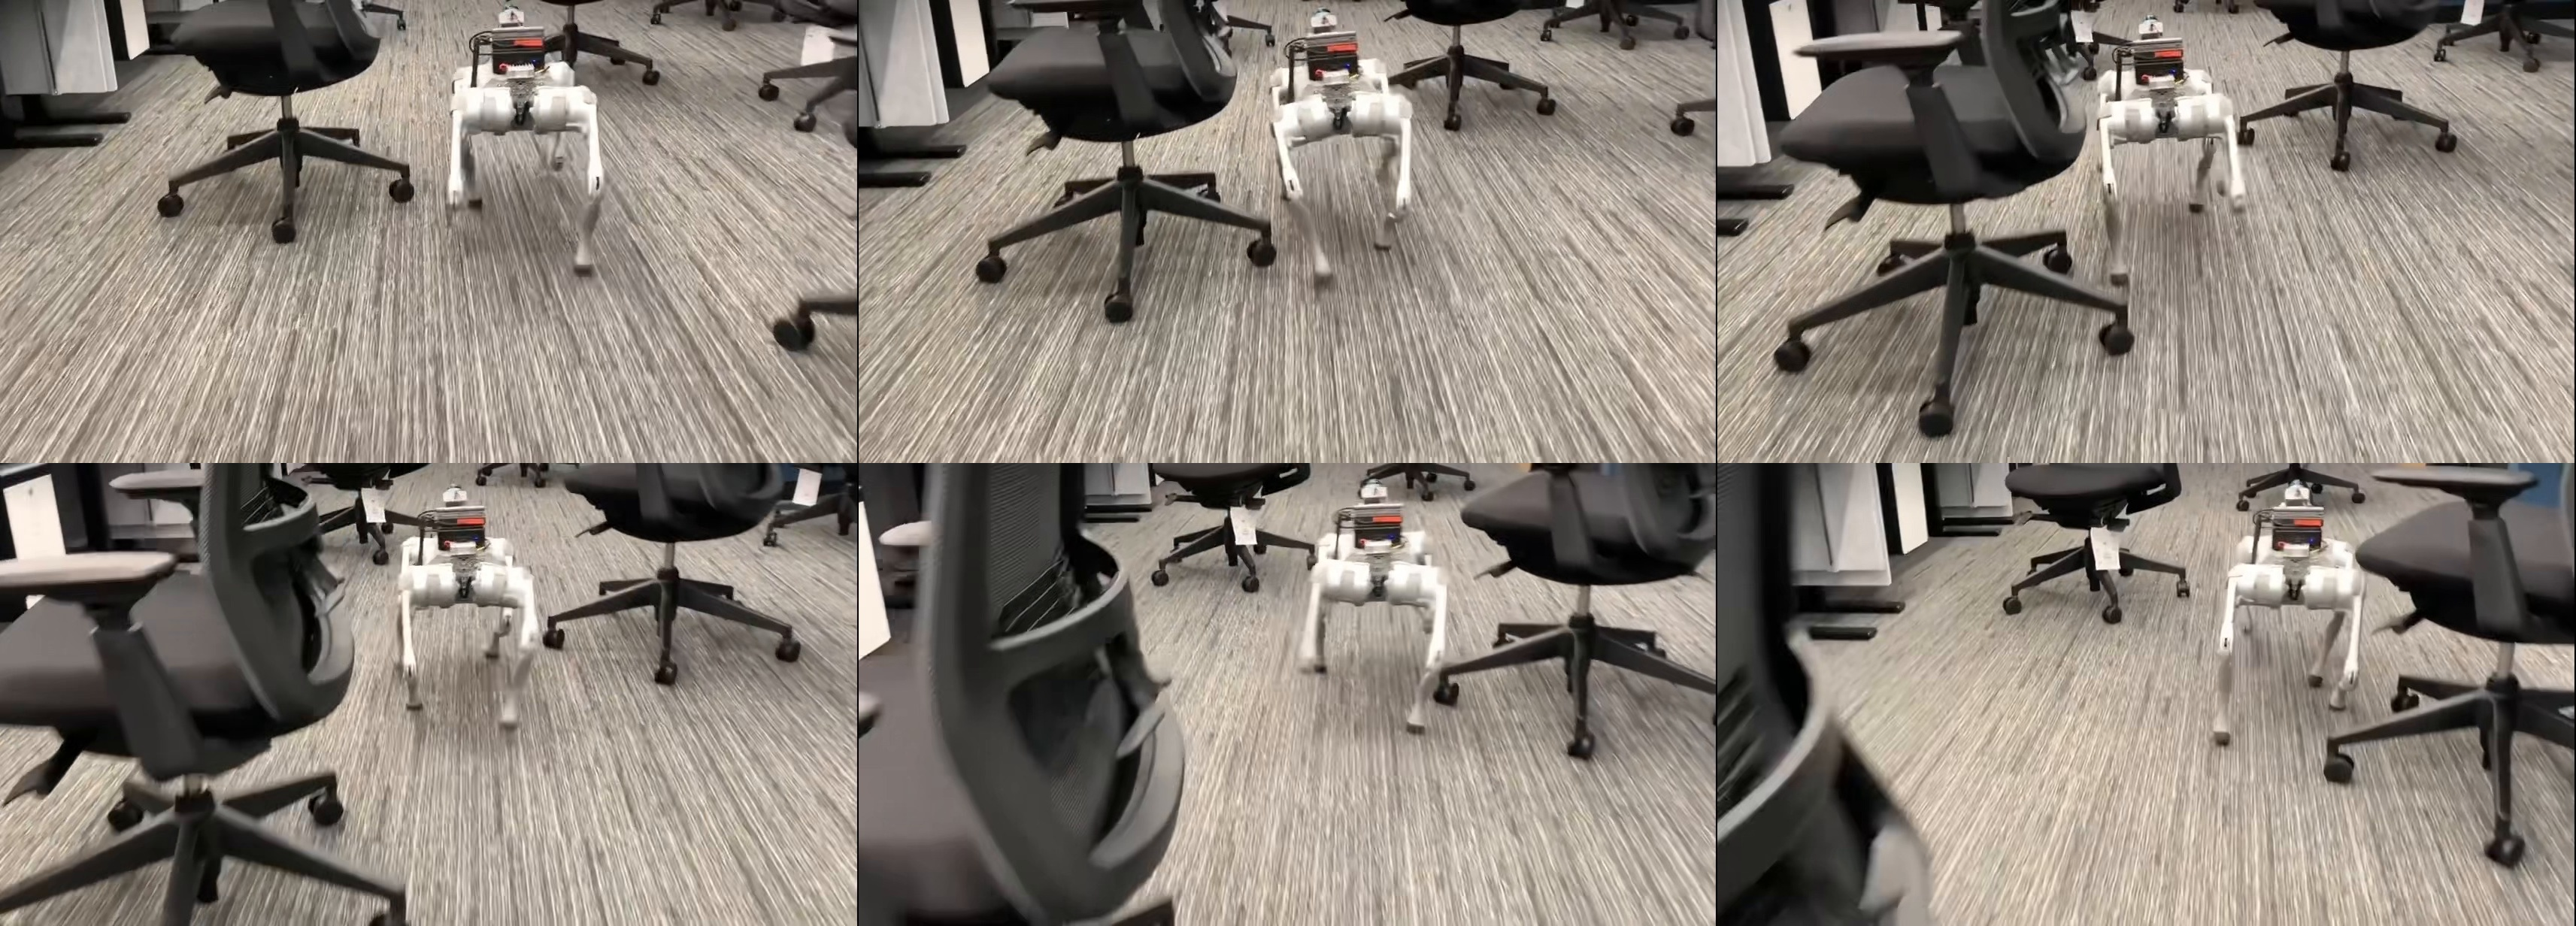
\includegraphics[width=\textwidth]{office_sequence_candidate_A.jpg}
\caption{Representative real-world deployment sequence showing the quadruped avoiding obstacles in a cluttered office environment.}
\label{fig:office_sequence}
\end{figure*}

As shown in Table~\ref{tab:ablation}, removing the hierarchical structure causes the most severe degradation, reducing the success rate from $70.8\%$ to $47.9\%$ while increasing the cost from $71.3$ to $116.7$. This reflects the difficulty of learning reach-avoid behavior directly in the high-dimensional joint-action space without the stabilized low-level motion interface. Removing the cost margin $\alpha$ primarily degrades budget feasibility, increasing BVR from $11.2\%$ to $22.4\%$, whereas removing the safety margin $\delta$ primarily degrades geometric safety, increasing CR from $18.6\%$ to $26.3\%$ and reducing MC from $0.32\,\mathrm{m}$ to $0.19\,\mathrm{m}$. Removing both margins further degrades safety and budget feasibility, and the overall ablation results indicate that the hierarchy, $\alpha$, and $\delta$ play complementary roles.

\subsection{Real-world Deployment}

We further deploy the learned policy on a Unitree Go2 robot in a cluttered office environment containing chairs, desks, and narrow passages. As illustrated in Figure~\ref{fig:office_sequence}, the robot is able to execute consecutive obstacle-avoidance maneuvers while maintaining stable locomotion under real-world sensing and actuation conditions.




















\section{Conclusion}

This paper formulated quadruped navigation as a minimum-cost reach-avoid problem and proposed \emph{HD-MCRA}, which combines a frozen low-level tracker, a nominal closed-loop abstraction, a budget-conditioned high-level policy, and conservative cost and safety corrections. This design makes augmented-state MCRA practical for quadruped navigation and achieves a better trade-off among success, safety, budget feasibility, and efficiency than the evaluated baselines. The ablation study further confirms that the hierarchy primarily improves success and reduces cost, while the conservative margins account for the gains in budget feasibility and geometric safety. While the present method adopts an engineering-oriented robust design, an important direction for future work is to place minimum-cost reach-avoid navigation for stochastic quadruped systems on firmer theoretical ground.

\bibliographystyle{IEEEtran}
\bibliography{references}









\end{document}
